
\section{mbiclique.rb 極大二部クリークの列挙\label{sect:mbiclique}}

本コマンドは、二部グラフから極大二部クリークを列挙する。
内部では\cite{UnoWeb}の\verb|lcm|コマンドを利用している。

$G=(V_1 \cup V_2,E)$を2つの部$V_1,V_2$の節点集合と部間の枝に張られた枝集合$E\subset V_1\times V_2$を持つ無向二部グラフとすると、
$V_1,V_2$の部分集合によって誘導される部分グラフの部間の任意の節点に枝があるような$G$の誘導部分グラフを二部クリークと呼ぶ。
%$V$の部分集合$V'$に対して$V'$によって誘導される部分グラフ$G'=(V',E(V'))(E'=\{(u,v) \in E|u,v \in V'\}$が完全グラフとなっている$G$の誘導部分グラフをクリークとい>う。
また、ある二部クリークが他の二部クリークの真部分集合でなければ、それは極大二部クリークと呼ばれる(図\ref{fig:biclique})。

\begin{figure}[htbp]
\begin{center}
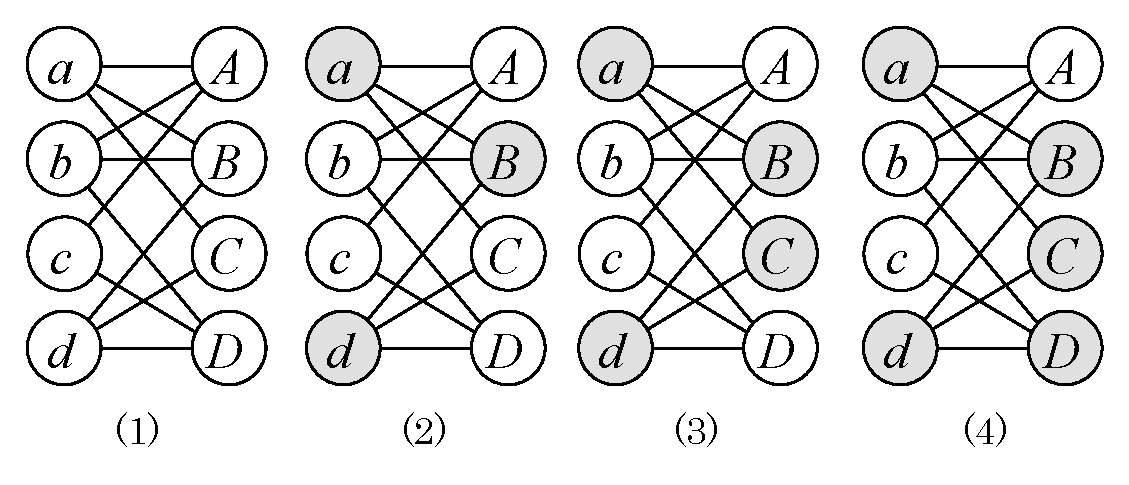
\includegraphics[scale=0.5]{./biclique.eps}
\caption{二部グラフ(1)について、網掛けで示された部分グラフ(2)は二部クリークではあるが、
(3)に示された二部クリークの真部分集合なので極大二部クリークではない。
一方で(3)はその他のどの二部クリークの真部分集合にはならないので極大である。
(4)は$a,D$間に枝がないので二部クリークではない。
\label{fig:biclique}}
\end{center}
\end{figure} 

極大二部クリークの列挙を使った応用例は多数考えられる。
例えば、消費者の食品購入パネルデータにおいて、一つの部を商品集合、他方の部を店集合と見なし、
ある閾値以上の購買のあった商品-店間に枝を張った二部グラフを構成できる。
そこから極大二部クリークを列挙することで、互いに強い関係にある商品と店のグルーピングが可能となる。

またテキストマイニングにおいては、格助詞句と用言句を各部と見なし、
用例のある格助詞句-用言句の間に枝を張った二部グラフを構成できる。
そこから極大二部クリークを列挙することで、互いに強い関係にある格フレーム(格助詞句-用言句ペアのこと)
のグルーピングが可能となり、ある種の概念を取得できる。

さらに、入札データにおいては、入札業者と案件をそれぞれ各部として考え、
実際に入札があった入札業者-案件の間に枝を張ることで二部グラフが構成できよう。

さて、本コマンドの入力データである二部グラフは、表\ref{tbl:bicl_input}に示されるような、
枝データを節点ペアとして表したCSV形式で与える(図\ref{fig:biclique} (1)に対応)。
項目が部を表している。
表\ref{tbl:bicl_input}では、小文字のアルファベットを要素として持つ\verb|node1|項目が一方の部を表し、
大文字のアルファベットを要素として持つ\verb|node2|項目が他方の部を表している。
グラフは無向グラフとして扱われ、島が複数あってもよい。

この二部グラフから極大二部クリークを列挙すると表\ref{tbl:bicl_output}に示されるような形式で
出力される。
一行が極大二部クリークに対応しており、各部を構成する要素が\verb|node1,node2|項目にベクトル形式で出力される。
\verb|size1,size2|には各部のサイズ(節点の数)が出力される。
5行目の極大二部クリーク($V_1=\{a,d\},V_2=\{B,C\}$)が図\ref{fig:biclique}(3)に対応している。
%また\verb|-node|オプションを指定することで
%\verb|node1,node2|項目にがクリークのIDで、この項目が同じ行で一つのクリークが識別される。
%\verb|id|=2のクリークが図\ref{fig:clique}(4)に対応し、
%\verb|id|=3のクリークが図\ref{fig:clique}(3)に対応している。
%その他にも、2つの節点から構成される極大クリーク$\{e,f\}$と$\{b,f\}$も列挙されている。
%最後の\verb|size|項目は、極大クリークを構成する節点数である。

\begin{table}[htbp]
\begin{center}
\begin{tabular}{cc}

\begin{minipage}{0.3\hsize}
\begin{center}
\caption{入力データ(枝データ)\label{tbl:bicl_input}}
{\small
\begin{tabular}{cc}
\hline
node1&node2 \\
\hline
a&A \\
a&B \\
a&C \\
b&A \\
b&B \\
b&D \\
c&A \\
c&D \\
d&B \\
d&C \\
d&D \\
\hline
\end{tabular} 
}
\end{center}
\end{minipage}

\begin{minipage}{0.3\hsize}
\begin{center}
\caption{出力結果\label{tbl:bicl_output}}
{\small
\begin{tabular}{llcc}
\hline
node1&node2&size1&size2 \\
\hline
a&A B C&1&3 \\
a b&A B&2&2 \\
a b c&A&3&1 \\
a b d&B&3&1 \\
a d&B C&2&2 \\
b&A B D&1&3 \\
b c&A D&2&2 \\
b c d&D&3&1 \\
b d&B D&2&2 \\
d&B C D&1&3 \\
\hline
\end{tabular} 
}
\end{center}
\end{minipage}

\end{tabular} 
\end{center}
\end{table} 

\subsection{書式}
\begin{verbatim}
書式) mbiclique.rb ei= ef= [o=] [l=] [u=] [T=] [-debug] [--help]

  ファイル名指定
  ei= : 辺データファイル
  ef= : 辺データ上の2つの節点項目名
  o=  : 出力ファイル
  l=  : 極大二部クリークを構成する最小節点数
      : ここで指定したサイズより小さい極大二部クリークは列挙されない。
      : カンマで区切って2つの値を指定すると、各部のサイズを制限できる。
      : カンマで区切った値の順番はef=で指定した項目の順番と同じ。
      : 制限を設けない場合は"l=2,"や"l=,2"のようにnull文字を指定する。
      : 後ろのnullは省略できる("l=2,"と"l=2"は同じ意味)。
  u=  : 極大二部クリークを構成する最大節点数
      : 指定の詳細はl=と同様である。

  その他
  T= : ワークディレクトリ(default:/tmp)
  --help : ヘルプの表示
\end{verbatim}

\subsection{注意点}
本コマンドの二部クリークの出力形式がベクトル形式(文字列を空白で区切った一つのCSV項目)となるため、
時に、一つの項目の長さが非常に長くなることがある。
そのため、内部で使っているMコマンドのCSV一行の最大長制約を超えてしまいエラーとなることがある。
そのようなときは、\verb|l=|もしくは\verb|u=|によって二部クリークのサイズを制約することで回避する。

\subsection{利用例}
\subsubsection*{例1: 基本例}

前節の解説で用いてる例。


\begin{Verbatim}[baselinestretch=0.7,frame=single]
$ more dat.csv
node1,node2
a,A
a,B
a,C
b,A
b,B
b,D
c,A
c,D
d,B
d,C
d,D
$ mbiclique.rb ei=dat.csv ef=node1,node2 o=result1.csv
#MSG# converting paired form into transaction form ...
#MSG# lcm_20140215 CIf /tmp/__MTEMP_95686_70245679198320_0 1 /tmp/__MTEMP_95686_7024567919
8320_3
trsact: /tmp/__MTEMP_95686_70245679198320_0 ,#transactions 4 ,#items 4 ,size 11 extracted 
database: #transactions 4 ,#items 4 ,size 11
 output to: /tmp/__MTEMP_95686_70245679198320_3
separated at 0
iters=11
11
1
3
4
3
#END# /usr/bin/mbiclique.rb ei=dat.csv ef=node1,node2 o=result1.csv
$ more result1.csv
node1,node2,size1,size2
a,A B C,1,3
a b,A B,2,2
a b c,A,3,1
a b d,B,3,1
a d,B C,2,2
b,A B D,1,3
b c,A D,2,2
b c d,D,3,1
b d,B D,2,2
d,B C D,1,3
\end{Verbatim}
\subsubsection*{例2: サイズを制限する例}

項目\verb|node1,node2|共にサイズが2の極大二部クリークを列挙する。


\begin{Verbatim}[baselinestretch=0.7,frame=single]
$ mbiclique.rb ei=dat.csv ef=node1,node2 o=result2.csv l=2,2 u=2,2
#MSG# converting paired form into transaction form ...
#MSG# lcm_20140215 CIf -l 2 -u 2 /tmp/__MTEMP_95739_70259512012180_0 1 /tmp/__MTEMP_95739_
70259512012180_3
trsact: /tmp/__MTEMP_95739_70259512012180_0 ,#transactions 4 ,#items 4 ,size 11 extracted 
database: #transactions 4 ,#items 4 ,size 11
 output to: /tmp/__MTEMP_95739_70259512012180_3
separated at 0
iters=10
4
0
0
4
#END# /usr/bin/mbiclique.rb ei=dat.csv ef=node1,node2 o=result2.csv l=2,2 u=2,2
$ more result2.csv
node1,node2,size1,size2
a b,A B,2,2
a d,B C,2,2
b c,A D,2,2
b d,B D,2,2
\end{Verbatim}
\subsubsection*{例3: 部分的にサイズを制限する例}

項目\verb|node1|のサイズの下限を1に(デフォルトの下限が1なので実際には意味がないが指定例として)、
項目\verb|node2|のサイズの上限を3に制限した極大二部クリークを列挙する。
\verb|u=|パラメータの1番目の値がnullになっているのは、項目\verb|node1|の上限を設定しなためである。



\begin{Verbatim}[baselinestretch=0.7,frame=single]
$ mbiclique.rb ei=dat.csv ef=node1,node2 o=result3.csv l=1, u=,3
#MSG# converting paired form into transaction form ...
#MSG# lcm_20140215 CIf -u 3 /tmp/__MTEMP_95792_70093564374420_0 1 /tmp/__MTEMP_95792_70093
564374420_3
trsact: /tmp/__MTEMP_95792_70093564374420_0 ,#transactions 4 ,#items 4 ,size 11 extracted 
database: #transactions 4 ,#items 4 ,size 11
 output to: /tmp/__MTEMP_95792_70093564374420_3
separated at 0
iters=11
11
1
3
4
3
#END# /usr/bin/mbiclique.rb ei=dat.csv ef=node1,node2 o=result3.csv l=1, u=,3
$ more result3.csv
node1,node2,size1,size2
a,A B C,1,3
a b,A B,2,2
a b c,A,3,1
a b d,B,3,1
a d,B C,2,2
b,A B D,1,3
b c,A D,2,2
b c d,D,3,1
b d,B D,2,2
d,B C D,1,3
\end{Verbatim}


